\documentclass[10pt]{article}
\usepackage[utf8]{inputenc}
\usepackage[english,russian]{babel}
\usepackage[T2A]{fontenc}
\usepackage{graphics}
\usepackage{graphicx}
\usepackage{amsmath,amssymb,amsthm,amsfonts,amscd}
\usepackage{float}
\usepackage{subfig}
\usepackage{algorithm}
\usepackage[noend]{algpseudocode}
\usepackage{hyperref}
\captionsetup[algorithm]{labelformat=empty}

\newtheorem{thm}{\indent Теорема}
\newtheorem{lem}{\indent Лемма}
\newtheorem{prop}{\indent Утверждение}
\bibliographystyle{unsrt}
\graphicspath{{../optimization/results/}}

\begin{document}
    \section{Введение}\label{sec:intro}
    Стационарная нормализированная диффузионная модель, описывающая радиационный и кондуктивный
    обмен в ограниченной области $\Omega \subset \mathbb{R}^3$ имеет следующий вид~\cite{modest-rht}
    \begin{equation}
        \label{initial}
        \begin{aligned}
            - a \Delta \theta + b \kappa_a(\theta ^ 3 | \theta | - \varphi) = 0,  \\
            - \alpha \Delta \varphi + \kappa_a (\varphi - \theta ^3 | \theta |) = 0.
        \end{aligned}
    \end{equation}
    Здесь $\theta$ – нормализованная температура,
    $\varphi$ – нормализованная интенсивность излучения, усредненная по всем направлениям.
    Положительные физические параметры $a, b, \kappa_a $ и $\alpha$,
    описывающие свойства среды, описываются следующим образом:
    \[
        a = \frac{k}{\rho c_v}, \; b = \frac{4 \sigma n^2 T^3_{\text{max}}}{\rho c_v}, \;
        \alpha = \frac{1}{3\kappa -A \kappa_s}
    \]
    где $k$ -- теплопроводность, $c_v$ -- удельная теплоёмкость, $\rho$ -- плотность,
    $\sigma$ -- постоянная Стефана\,--\,Больцмана, $n$ -- индекс рефракции,
    $T_{\text{max}}$ -- максимальная температура, $\kappa := \kappa_s + \kappa_a$ -- коэффициент
    полного взаимодействия, $\kappa_s$ -- коэффициент рассеяния.
    Коэффициент $A \in [-1,1]$ описывает анизотропию рассеивания;
    случай $A=0$ отвечает изотропному рассеиванию.

    Далее будем считать, что функция $\theta$ удовлетворяет следующему условию на границе
    $\Gamma = \partial \Omega$:
    \begin{equation}
        \label{theta-dirichlet}
        \theta|_\Gamma = \theta_b.
    \end{equation}
    Для задания сдандартного краевого условия для интенсивности излучения $\varphi$ обычно
    используют граничное условие вида
    \begin{equation}
        \label{phi-default}
        - \alpha \partial_n \varphi + \gamma (\varphi - \theta ^4) = 0.
    \end{equation}
    Здесь и далее $\partial_n$ обозначает производную в отношении внешней нормали.
    В случае если функция $\gamma$ не известна, естественно вместо краевого условия для
    интенсивности излучения задать значение теплового потока на границе
    \begin{equation}
        \label{theta-neumann}
        \partial_n \theta = q_b.
    \end{equation}
    Численное решение
    задачи~\eqref{initial},~\eqref{theta-dirichlet},~\eqref{theta-neumann},
    на которую мы будем ссылаться как на задачу $P$, является затруднительным из-за необходимости
    решать дифференциальное нелинейное уравнение четвёртого порядка.
    Теоретический анализ и доказательство существования решения задачи $P$ представлено
    в~\cite{cheb-same}.
    Одним из подходов к решению может быть замена исходной задачи $P$ на задачу
    оптимального управления.
    За функцию управления возьмём функцию $u$ такую, что
    \begin{equation}
        \label{phi-neumann}
        \partial_n \varphi |_\Gamma = u.
    \end{equation}
    Из граничных условий ~\eqref{theta-neumann},~\eqref{theta-dirichlet} получим
    \begin{equation}
        \label{theta-neumann-r}
        \partial_n \theta  + \theta - r = 0, \;\; r := q_b + \theta_b.
    \end{equation}
    Задача оптимального управления заключается в минимизации функционала качествa
    \begin{equation}
        \label{quality}
        J(\theta, u) = \frac{1}{2} ||\theta - \theta_b||^2_\Gamma + ||u||^2_\Gamma,
    \end{equation}
    Обозначим~\eqref{initial},~\eqref{phi-neumann},~\eqref{theta-neumann-r},~\eqref{quality}
    как задачу оптимального управления $CP$.


    Исследование ...
    %    математических моделей радиационного теплопереноса [1], учитывающих одновременно
    %    вклад эффектов теплопроводности и излучения даёт теоре-тическую основу для инженерных решений
    %    в различных областях, таких как произ-водство стекла [2],
    %    лазерная интерстициальная термотерапия [3], и др.
    %    Главной особенностью данных процессов является существенное влияние излучения на теплообмен
    %    при высоких температурах.
    %    Значительное число работ посвящено исследованиюзадач управления для
    %    нестационарных моделей сложного теплообмена [4–6], в ко-торых для описания температурного поля
    %    используется нестационарное уравнениетеплопроводности, а для моделирования излучения --
    %    стационарное диффузионноеприближение уравнения переноса излучения.
    %    В работах [7, 8] задача оптимального управления сводится к
    %    bang-bang принципу [9], или аналогичному.
    %    Близкая к рассмотренной в данной статье задача управления коэффициентом отражения
    %    для полностью стационарной модели исследовалась в [10],
    %    для нестационарной модели – в [11].
    %    Отметим также работы [12, 13], в которых рассмотрены свойства квазирешений
    %    обратных задач для уравнений тепломассапереноса.

    \section{Формализация задачи нахождения квазирешения}\label{sec:formalization}
    будем предполагать, что исходные данные удовлетворяют следующему условию:

    (i) WIP\@.

    Пусть $H = L^2(\Omega), V = W^1_2(\Omega), Y = V \times V $.
    Пространство $H$ отождествляем с сопряжённым пространством $H'$ так,
    что $V \subset H = H' \subset V'$.
    Определим $(f,v)$ как значение функционала $f \in V'$ на элементе $v \in V$,
    совпадающее со скалярным произведением в $H$, если $f\in H, \|f\|^2 = (f,f)$.
    Пространство $U = L^2(\Gamma)$ является пространством управлений;


    Пусть $v$ произвольный элемент множества $H^1(\Omega)$.
    Определим операторы:

    \begin{gather*}
        A_{1,2}\colon V \to V', \;\; F \colon V \times U \to V', \; f \in V', \; g \in V'.\\
        (A_1\theta,v) = a( \nabla \theta, \nabla v ) + \int_\Gamma a \theta v d\Gamma, \;
        (A_2 \varphi, v) = \alpha (\nabla \varphi,\nabla v), \\
        (f,v) = \int_\Gamma r v d\Gamma, \;\; (g,v) = \int_\Gamma \alpha u v d\Gamma,\\
    \end{gather*}

    Пару $\{\theta, \varphi \} \in Y$ будем называть слабым решением
    задачи~\eqref{initial},~\eqref{phi-neumann},~\eqref{theta-neumann-r} если
    \begin{equation}
        \label{weak-operational}
        A_1 \theta + b \kappa_a (| \theta | \theta^3 - \varphi ) = f,
        A_2 \varphi + \kappa_a (\varphi - |\theta|\theta^3)  = g.
    \end{equation}

    Задача нахождения оптимального управления состоит в минимизации функционала $J(\theta, u)$,
    определённом на паре $\theta, u$, где $\theta$ -- компонент
    решения системы~\eqref{weak-operational}.
    Таким образом
    \begin{equation}
        \label{minimization-operational}
        J(\theta, u) \to \text{inf}, \; \{\theta, \varphi\}
        \text{ решение~\eqref{weak-operational}, соответствующее функции } u \in U.
    \end{equation}

    Пара $\{\hat{\theta}, \hat{\varphi} \}$ соответствующая минимуму $J$,
    отвечающая функции $\hat{u}$ называется оптимальным состоянием.

    \section{Анализ решения экстремальной задачи}\label{sec:analysis}
    \begin{thm}
        \label{cp-existing}
        Пусть выполняются условия (i).
        Тогда существует решение задачи $CP$.
    \end{thm}
    \begin{proof}
        wip.
    \end{proof}

    Вывод условий оптимальности основан на принципе множителей
    Лагранжа для гладко-выпуклых задач минимизации.
    \begin{thm}
        \label{adjoint_theorem}
        Пусть $\hat{y}=\{\hat{\theta},\hat{\varphi} \} \in Y, \hat{u} \in U_{ad}$ --- решение
        экстремальной задачи~\eqref{minimization-operational}.
        Тогда существует пара $p = (p_1, p_2)$, $p \in Y$
        такая, что тройка $(\hat{y}, \hat{u}, p)$, удовлетворяет следующим условиям:
        \begin{equation}
            \label{theorem_2_eq1}
            A_1 p_1 + 4 |\hat{\theta}|^3 \kappa_a(b p_1 - p_2) = f_c, \;\;
            (f_c,v) = - \int_{\Gamma_2} (\hat{\theta} - \theta_0) v d\Gamma,
        \end{equation}
        \begin{equation}
            \label{theorem_2_eq2}
            A_2 p_2 + \kappa_a (p_2-b p_1) = g_c(( p_2, \hat{u}),v), \;\;
            g_c(( p_2, \hat{u}),v) = -\int_{\Gamma_1} \hat{u} p_2 v\Gamma,
        \end{equation}
        \begin{equation}
            \label{theorem_2_eq3}
            \int_{\Gamma_1} p_2 (\hat{\varphi} - \theta_b^4)(u-w) \leq 0
            \quad \forall w \in U_{ad}.
        \end{equation}
    \end{thm}
    \begin{proof}
        %        Перепишем уравнения~\eqref{weak-operational} следующим образом:
        %        \begin{gather*}
        %            H(y,u) = 0,\;\; y = \{\theta,\varphi\} \in Y, \; \text{где}\\
        %            H:Y \times U \to Y',\\
        %            H(y,u) =\{A_1 \theta + b \kappa_a (| \theta | \theta^3 - \varphi ) - f,
        %            A_2 \varphi + \kappa_a (\varphi - |\theta|\theta^3) + F(\varphi, u) - g \}.\\
        %        \end{gather*}
        %        Заметим, что для всех $u \in U_{ad}$, отображение $y \to J(\theta) $ и $y \to H(y,u)$
        %        непрерывно дифференцируемо в окрестности $\mathcal{O}(\hat{y})$ точки $\hat{y}$.
        %        Непрерывная дифференцируемость членов в $H$ следует из непрерывной дифференцируемости
        %        функции $t \in \mathbb{R} \to | t | t^3$, а также из непрерывности вложения
        %        $V \subset L^6(\Omega)$.
        %        В дополнение, отображение $u \to H(y,u)$ непрерывно из $U \to Y'$ и афинно.
        %        В~\cite{cheb_origin} показано, что $\text{Im}H_y'(\hat{y}, \hat{u}) = Y$,
        %        что влечёт невырожденность условий оптимальности.
        %
        %        Рассмотрим функцию Лагранжа
        %        $L(y,u,p) = J(\theta) + (H(y,u),p)$, где $y,p \in Y,\, u \in U_{ad}$.
        %        Согласно принципу Лагранжа \cite[Гл.2, Теорема 1.5]{theorem_proof_18}
        %        существует пара $p = \{p_1,p_2\} \in Y$ такая, что
        %        \begin{equation}
        %            \label{th2_proof_1}
        %            (L_\theta,\zeta) =\int_{\Gamma_2}(\hat\theta -\theta_0) \zeta d\Gamma +
        %            (A_1 \zeta + 4b\kappa_a |\hat\theta|^3 \zeta,p_1) -
        %            4\kappa_a(|\hat\theta|^3 \zeta,p_2) = 0 \; \forall \zeta \in V,
        %        \end{equation}
        %        \begin{equation}
        %            \label{th2_proof_2}
        %            (L_\varphi, \zeta) = (A_2 \zeta + \kappa_a \zeta, p_2) -
        %            b \kappa_a(\zeta,p_1) +\int_{\Gamma_1} \hat u \zeta p_2 = 0 \; \forall \zeta \in V,
        %        \end{equation}
        %        \begin{equation}
        %            \label{th2_proof_3}
        %            (L_u,\tau) = \int_{\Gamma_1} \tau (\varphi - \theta^4_b) p_2 d\Gamma  \leq 0, \;
        %            \tau := \hat u - w \; \forall w \in U_{ad}.
        %        \end{equation}

        \@. WIP.
    \end{proof}

    \section{Численные эксперименты}\label{sec:experiments}

    Пусть функционал $J(\theta)$ удовлетворяет условиям, указанным в \autoref{sec:optimality}.
    Для удобства введём переобозначение
    $\hat{J}(u):=J(\theta(u)), \hat{J}:L^2(\Gamma_1) \to \mathbb{R}$.
    Здесь $\theta(u)$ -- температурное поле задачи~$CP$ отвечающее управлению $u \in L^2(\Gamma)$.
    Согласно формуле~\eqref{theorem_2_eq3} градиент функционала $\hat{J}(u)$
    имеет вид
    \[ hat{J}'(u)= \epsilon u - p_2, \]
    где $p_2$ -- соответствующая переменная сопряжённой системы.

    Предлагаемый алгоритм решения выглядит следующим образом:
    \begin{algorithm}[H]
        \caption{Алгоритм градиентного спуска с проекцией}
        \begin{algorithmic}[1]
            \State Выбираем значение градиентного шага $\lambda$,
            \State Выбираем количество итераций $N$,
            \State Выбираем произвольное $u_0 \in U$,
            \For{$k \gets 0,1,2,\ldots,N$}:
            \State Для полученного $u_k$ расчитываем состояние
            \State Расчитываем значение функционала качества $J(\theta_k)$ из \eqref{quality}.
            \State Расчитываем сопряжённое состояние $p_k=\{p_{1k},p_{2k}\}$ из
            уравнений~\eqref{theorem_2_eq1}--\eqref{theorem_2_eq2},
            где $ \hat{\theta} := \theta_k, \hat{u}=u_k$.
            \State Пересчитываем управление
            $u_{k+1} = P_{ad}\left[ u_k - \lambda (\varphi_k - \theta_b^4)p_{2k} \right]$.
            \EndFor
        \end{algorithmic}
    \end{algorithm}
    Приведём далее примеры расчётов для двумерного случая.
    Положим $\Omega = \{(x,y), 0 \leq x,y \leq 1\}$, $l = 1$ см.
    Будем далее считать, что $a = 0.006[\text{см}^2/\text{c}]$, $b=0.025[\text{см}/\text{с}]$,
    $\beta = 0.00005[\text{см}/\text{с}]$, $\kappa=1[\text{см}^{-1}]$, $\kappa_s = 0$, $A = 0$,
    $\gamma = 0.3$.
    Указанные параметры соответствуют стеклу~\cite{grenkin_13}.
    Температуру на границе $\Omega$ положим равной $\theta_b = ???$.

    При указанных параметрах для первого эксперимента выберем следующее начальное значение
    функции $u$ (рис.~\ref{control}\subref{fig1:exp1}):
    \begin{equation}
        \label{test_function_1}
        u(x)= sin(x) * y
    \end{equation}
    и для второго эксперимента (рис.~\ref{control}\subref{fig1:exp2}):
    \begin{equation}
        \label{test_function_2}
        u(x)=0.49x+0.01.
    \end{equation}

    Далее, применяя предложенный алгоритм решаем задачу оптимального управления $CP$.
    Эффективность алгоритма, а также значение $u_0$
    в первом и втором случаях иллюстрируются рис.~\ref{control}.
    На рис.~\ref{cost} показана динамика функционала качества по итерациям.

    \begin{figure}[H]
        \centering
        \subfloat[Первый эксперимент]
        {
        \label{fig1:exp1}
        \includegraphics[width=.51\linewidth]{../optimization/results/init_control.png}
        }
        \subfloat[Второй эксперимент]
        {
        \label{fig1:exp2}
        \includegraphics[width=.51\linewidth]{../optimization/results/control.png}
        }
        \caption{Тестовая функция $u$, начальная $u_0$, найденная функция $u_{end}.$}
        \label{control}
    \end{figure}

    \begin{figure}[H]
        \centering
        \subfloat[Первый эксперимент]
        {
        \label{fig2:exp1}
        \includegraphics[width=.51\linewidth]{../optimization/results/theta.png}
        }
        \subfloat[Второй эксперимент]
        {
        \label{fig2:exp2}
        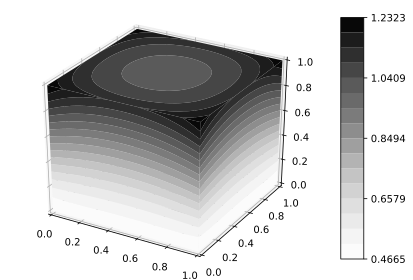
\includegraphics[width=.51\linewidth]{../optimization/results/phi.png}
        }
        \caption{Динамика функции $\hat{J}(u)$ по итерациям.}
        \label{cost}
    \end{figure}


    \bibliography{bibliography}

\end{document}

